\documentclass[12pt,letterpaper]{article}
\usepackage{fullpage}
\usepackage[top=2cm, bottom=4.5cm, left=2.5cm, right=2.5cm]{geometry}
\usepackage{amsmath,amsthm,amsfonts,amssymb,amscd}
\usepackage{lastpage}
\usepackage{enumerate}
\usepackage{fancyhdr}
\usepackage{mathrsfs}
\usepackage{xcolor}
\usepackage{graphicx}
\usepackage{hyperref}
\usepackage{sectsty}
\usepackage{enumitem}
\usepackage{siunitx}
\usepackage{subfig}
\usepackage{stackengine}


\sectionfont{\fontsize{14.4}{17}\selectfont}
\subsectionfont{\fontsize{12}{12}\selectfont}

\hypersetup{%
  colorlinks=true,
  linkcolor=blue,
  linkbordercolor={0 0 1}
}

\setlength{\parindent}{0.0in}
\setlength{\parskip}{0.05in}

% Edit these as appropriate
\newcommand\course{EEEE 380}
\newcommand\hwnumber{2}
\newcommand\NetIDa{Andrei Tumbar}

\pagestyle{fancyplain}
\headheight 35pt
\lhead{\NetIDa}
\chead{\textbf{\Large Exam \hwnumber}}
\rhead{\course \\ \today}
\lfoot{}
\cfoot{}
\rfoot{\small\thepage}
\headsep 1.5em

\newcommand\ddfrac[2]{\frac{\displaystyle #1}{\displaystyle #2}}

\newcommand{\capequation}[1]{\begin{center} #1 \end{center}}

\begin{document}

\section*{RTL inverters}

\begin{figure}[h!]
  \centering
  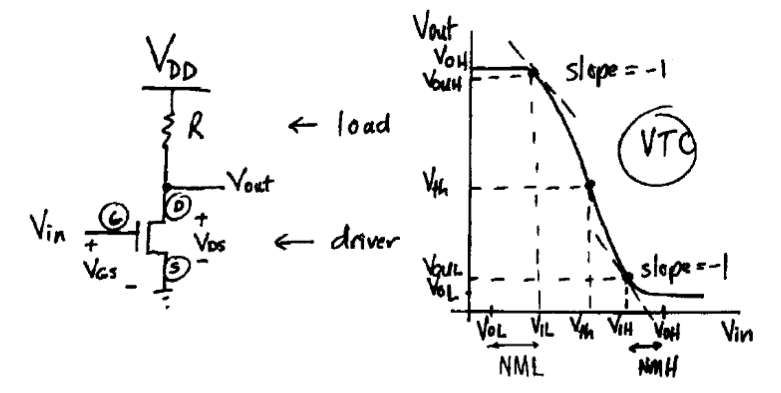
\includegraphics[width=5.5in]{rtl_vtc.png}
  \caption{RTL VTC}
  \label{fig:pa}
\end{figure}

\begin{equation}
\frac{V_{DD} - V_{out}}{R} = \frac{k_n}{2}(E_{CN}L_N)\frac{(V_{th} - V_{TN})^2}{V_{th} - V_{TN} + E_{CN}L_N}
\end{equation}
\capequation{SCM model of $V_{th}$}

\begin{equation}
\frac{V_{DD} - V_{out}}{R} = \frac{k_n}{2}(V_{th} - V_{TN})^2
\end{equation}
\capequation{LCM model of $V_{th}$}

Noise margin low (NML) = $V_{IL} - V_{OL}$ \\
Noise margin high (NMH) = $V_{OH} - V_{IH}$

\subsection*{$V_{OL}$}
\begin{equation}
\ddfrac{k_n}{1+\frac{V_{OL}}{E_{CN}L_N}}\left[(V_{DD}-V_{TN})V_{OL} - \frac{{V_{OL}}^2}{2}\right] = \ddfrac{V_{DD} - V_{OL}}{R}
\end{equation}
\capequation{SCM model of $V_{OL}$}

\begin{equation}
V_{OL} = \frac{V_{DD}}{1 + k_nR(V_{DD} - V_{TN})}
\end{equation}
\capequation{LCM model of $V_{OL}$}

\section*{CMOS Inverter}

\begin{figure}[h!]
  \centering
  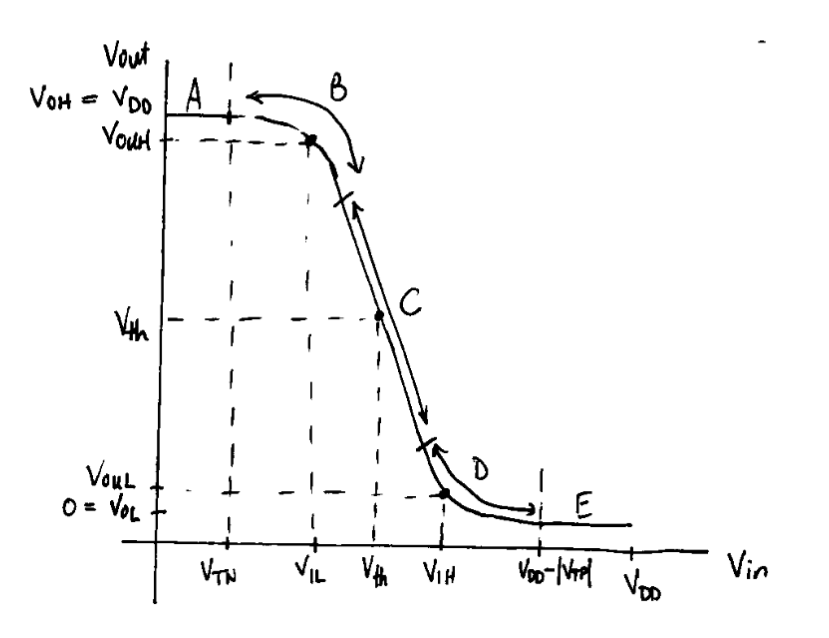
\includegraphics[width=5.5in]{cmos_vtc.png}
  \caption{CMOS VTC}
  \label{fig:pa}
\end{figure}

\begin{table}[h!]
    \renewcommand{\arraystretch}{1.3}
    \setlength{\tabcolsep}{12pt}
    \begin{center}
        \begin{tabular}{|c|c|c|}\hline
        Range & PMOS & NMOS\\\hline
        A & OFF & ON \\\hline
        B & SAT & TRI \\\hline
        C & SAT & SAT \\\hline
        D & SAT & TRI \\\hline
        E & ON & OFF \\\hline
        \end{tabular}
    \end{center}
    \label{tab:tim}
\end{table}

\end{document}
